\documentclass[12pt]{article}

\usepackage{xspace}
\usepackage{lineno}
\usepackage{setspace}
\usepackage{graphicx}
\usepackage{subfigure}
\usepackage{float}
\usepackage{color}
\usepackage{caption}
\usepackage[margin=1in]{geometry}
\usepackage{natbib}
\usepackage{amsmath}
\usepackage{hyperref}


%\setlength{\marginparwidth}{1in}
\let\oldmarginpar\marginpar
\renewcommand\marginpar[1]{\-\oldmarginpar[\raggedleft\tiny #1]%
{\raggedright\tiny #1}}

\begin{document}
\doublespacing
\linenumbers

\newcommand{\kluyveri}{\emph{L. kluyveri}\xspace}
\newcommand{\Lklu}{\emph{L. kluyveri}\xspace}
\newcommand{\dubl}{\emph{C. dubliniensis}\xspace}
\newcommand{\gossypii}{\emph{E. gossypii}\xspace}
\newcommand{\ROC}{ROC SEMPPR\xspace}
\newcommand{\GC}{GC content\xspace}
\newcommand{\DM}{\ensuremath{{\Delta M}}\xspace}
\newcommand{\DE}{\ensuremath{{\Delta \eta}}\xspace}

\newcommand{\beginsupplement}{%
        \setcounter{table}{0}
        \renewcommand{\thetable}{S\arabic{table}}%
        \setcounter{figure}{0}
        \renewcommand{\thefigure}{S\arabic{figure}}%
     }

\noindent RH: LANDERER ET AL.--- Intragenomic variation in codon usage
% put in your own RH (running head)
% for POVs the RH is always POINT OF VIEW
\bigskip
\medskip
\begin{center}

% Insert your title:
\noindent{\Large \bf Decomposing mutation and selection to identify mismatched codon usage}
\bigskip

% We don't use a special title page; the author information is entered
% like any other text.

% FOOTNOTES: We don't allow them in the manuscript, except in
% tables. Don't include any footnotes in the text.


\noindent{C\textsc{EDRIC} ~{L\textsc{ANDERER}}$^{1,2,*}$,
R\textsc{USSELL} {Z\textsc{ARETZKI}}$^{3}$,
\textsc{AND}
M\textsc{ICHAEL} A.~{G\textsc{ILCHRIST}}$^{1,2}$}

\end{center}

\vfill

{\small
\noindent$^{1}$Department of Ecology \& Evolutionary Biology, University of Tennessee, Knoxville, TN 37996-1610\\
\noindent$^{2}$National Institute for Mathematical and Biological Synthesis, Knoxville, TN 37996-3410\\
\noindent$^{3}$Department of Business Analytics \& Statistics, Knoxville, TN ~ 37996-0532 \\
\noindent$^{*}$Corresponding author. E-mail:~cedric.landerer@gmail.com
}

\vfill
\centerline{Version dated: \today}
\vfill
\newpage

\begin{abstract}
Here we examine variation in codon usage patterns of endogenous and exogenous genes in the yeast \emph{Lachancea kluyveri}.
Previous studies indicate that the left arm of chromosome C, or $\sim 10 \%$ of the \Lklu genome, is the result of an large introgression of exogenous genes.
Thus, the \Lklu genome provides an opportunity to study the adaptation of these exogenous to a novel cellular environment and estimate how the genetic load of these genes changes over time.
In order to quantiatively describe \Klu's codon usage environment, we fitted a bayesian, mechanistic model of codon usage bias evolution, ROC-SEMPPR, to \Klu's endogenous gene in order to estimate the strength of mutation bias and selection on codon usage.
We then compared these parameter estimates to those we obtained by fitting ROC-SEMPPR to \Klu's exogenous genes, which provides a biased estimate of the ancestral environment of the exogenous genes.
Our results indicate the differences in codon usage between \Klu's endogenous and exogenous genes are largely due to differences in mutation bias, rather than selection.
% differences from A/T ending codons in the endogenous genes to C/G ending codons in the exogenous genes
Estimating mutation and selection parameters separately for the endogenous and exogenous genes improved our ability to predict empirical estimates of protein synthesis by 17\% and avoided errors in identifying \Klu's selectively favored or `optimal' codons.
By comparing our mutation and selection parameters to those estimated for other yeast species, we identified \emph{Eremothecium gossypii} as the most likely source of \Klu's exogenous genes.
Using these parameters and available estimates of mutation rates in yeast, we estimated the age of the introgression to be on the order of $6\times 10^8$ generation.
Finally, we estimated the genetic load of the exogeneous genes both at the time of introgression and currently.
In summary, our work shows the advantage of using mechanistic models that separate the effects of selection and mutation on codon usage.
\end{abstract}
\newpage


\section*{Introduction}
Synonymous codon usage patterns often varies within a genome and between taxa and reflects the effects of mutation bias, selection, and genetic drift.
The signature of mutation bias is largely determined by the organism's internal or cellular environment, such as their complement DNA repair genes.
The signature of selection on codon usage is also largely determined by an organism's cellular environment, such as its translational machinery. 
In contrast, the strength of selection on the codon usage of an individual gene is largely determined by its expression level which, in turn, is largely determined by the organism's external environment.
The efficacy of this selection on codon usage relative to drift is a function of the organism's effective population size \Ne which, in turn, is largely determined by its external environment.
Thus, the codon usage patterns of a genome provides us with a unique signature of the organism's internalby decomposing the patterns codon usage bias across a set of genes allows us to genome provides us with information about the organism's cellular and external environment.

In general, the strength of selection on codon usage increases with gene expression \citep{ikemura1985, gouy1982}.
Conversely, the impact of mutation bias on codon usage declines with gene expression.
Thus, we can easily imagine that with increasing gene expression, codon usage shifts from a process dominated mutation to a process dominated by selection.
Together, the mutation process favoring specific synonymous codons - or mutation bias -  and the selection for translation efficiency scaled by gene expression and effective population size - or selection bias -  shape codon usage in a genome.
This mutation-selection-drift balance model allows us to explicitly describe the environment in which genes evolve with respect to mutation and selection bias.
Here we show that estimating the influence of mutation bias and selection bias on a gene's codon usage allows us to not only predict protein synthesis rate $\phi$, but also, to infer its history and make predictions about its future with respect to these forces.

Most studies implicitly assume that synonymous codon usage of a genome is reflects the single mutational and selective cellular environment of the organism. 
However, any introgressed genes, whether the result of hybridization or horizontal gene transfer, should carry the signature of the exogenous cellular environment whence they came and, in turn, impose a genetic load on the recipient lineage.
The magnitude of the exogenous genes' genetic load on the recipient or endogenous lineage should increase as the mutation and selective environments differ between the donor and recipient lineages as well as with the expression level of the genes in the recipient cells.
Thus codon usage patterns likely play a critical role in the rates of introgression between lineages and, as a result, can serve as an important source of information about such events.

Here we analyze the synonymous codon usage of the genome of \emph{Lachancea kluyveri}, the earliest diverging lineage of the Lachancea clade.
The Lachancea clade diverged from the Saccharomyces clade prior to the whole genome duplication, about 100 Mya ago.
Since its divergence from the other Lachancea, \kluyveri  has experienced a large introgression of exogenous genes.
These introgressed exogenous genes replaced XXXX genes, constituting the entire left arm of \Klu's C chromosome, and were identified due to their $\sim13\%$ elevation in \GC bias relative to the remaining, endogenous genes of the \Klu genome \citep{payen2009, friedrich2015}.

In order to study the effects of introgression and the resulting mismatches in codon usage in the \Klu genome,  we use \ROC, a mechanistic model of codon usage bias evolution grounded in population genetics.
\ROC, which uses a bayesian MCMC method for model fitting,  allows us to quantify the contributions of mutation bias and selection on to the codon usage patterns of a set of genes.
\ROC also allows us to predict a gene's average predicting protein production rate based on its individual codon usage pattern with a precision comprable to that of more direct empirical methods \citep{gilchrist2015}.
By fitting \ROC separately to \Klu's endogenous and exogenous sets of genes we generate a quantiative description of their signatures of mutation bias and natural selection for efficient protein translation.
Our results indicate that the difference in \GC between endogenous and exogenous genes mostly to differences in mutation bias.
In addition, we show that separately fitting \ROC to endogenous and exogenous gene sets substantially improves our ability to predict empirical estimates of protein synthesis rates over fitting ROC to a combined dataset of endogenous and exogenous genes.

In order to identify a potential source lineage for \Klu's exogenous gene set we fit \ROC to the genomes of 38 yeastspecies.
We then compared ROCs parameter estimates of mutation bias and selection of \Klu's exogenous genes to these species and found a strong correlation in only two species, \gossypii and \dubl.
We also compared the synteny of \Klu's exogenous genes to these lineages.
We found strong synteny in a number of cases, most notably in \gossypii but not \dubl.
As a result, we conclude that of the yeast species we examined, the \gossypii lineage is most closely related to the the donor of \Klu's exogenous genes.
Assuming that \gossypii's mutation bias is similar to the source of the exogenous genes, we estimated the introgression occurred approximately $6 \times 10^8$ generations ago using a model of exponential decay to describe the  shift in mutation bias of the exogenous genes.
Finally, we estimate the selective cost or genetic load of the exogenous genes due to codon usage mismatch using our estimates of the selection parameters from \Klu's endogenous genes and the our estimates of the protein synthesis rate of the exongenous genes.
%Thus, in addition to being able to estimate codon preference and gene expression to describe codon usage patterns, we also gain insights into the evolution of genes that have been transferred between lineages.

Need to discuss introgression
\begin{itemize}
\item Load calculations 
  \begin{itemize}
  \item Some genes pre-adapted to new environment
  \item Most genes not
  \item Load estimate indicates strong selection against introgression sequences alone
  \end{itemize}
\item Explaining introgression
  \begin{itemize}
  \item Assuming introduction is continuous as it appears, indicates little recombination during spread
  \item Data suggests introgression spread quickly
  \item Potential explanations
    \begin{itemize}
    \item Major flaws in our calculation of fitness costs.
      For example, if the relationship between expression and fitness is flat, then CU cost could be reduced if expression is reduced.
    \item Introgression triggered speciation event, thus \Ne was very small ($<100$) so even if strongly selected against it still had a reasonable probability of fixing. 
    \item Strong selection on coding or regulatory sequence at one or more loci countered selection on CU
    \item Unlikely event, but introgressions happen frequently.
      Note here mutation is actually an introgression event, not a nt change.
      Although pop gen predicts fixation probability is very low.
      However, pop gen also tells us that if such an unlikely fixation occurs, it is very likely to happen quickly.
      Thus, continuous nature of introgression also consistent with a rare, maladaptive fixation event.
    \item Other adaptive effects of introgression seems most plausible, but since we don't know have reasonable estimates about frequently hybridiations occur nor accurate estimate of how frequent such introgressions fix, the maladaptive explanation is hard to evaluate.
    \item Combination of most maladaptive, some adaptive alleles, and speciation could also be a feasible hypothesis.
    \end{itemize}
  \end{itemize}
\end{itemize}
\section*{Results}
Model selection and validation confirmed that the \kluyveri genome contains signatures of at least two cellular environments.
We compared model fits of \ROC to the homogeneous \kluyveri genome and the separated sets of endogenous and exogenous genes of 4864 and 497 genes respectively, using AnaCoDa \citep{landerer2018}.
We compared estimates of the cellular environment to describe differences in endogenous and exogenous codon usage.
Furthermore, we utilize the differences in model fit and parameters estimated from the endogenous and exogenous genes to explore the evolution of the exogenous gene set.

AIC indicates that parameter estimates for mutation bias (\DM) and selection bias (\DE) differ greatly between exogenous and endogenous gene sets.
As a result, the partitioning of the \kluyveri genome into an endogenous and exogenous gene set is clearly favored by model selection.
The inclusion of 81 additional parameters ($40$ for \DM, $40$ for \DE, and one for $s_{\phi}$) necessary to describe both gene sets separately improves our model fit by $\sim 78,000$ AIC units (5,313,110 for the combined gene set vs 5,235,598 for the separated gene sets).

\begin{figure}[t]
    \centering
    \begin{subfigure}
        \centering
        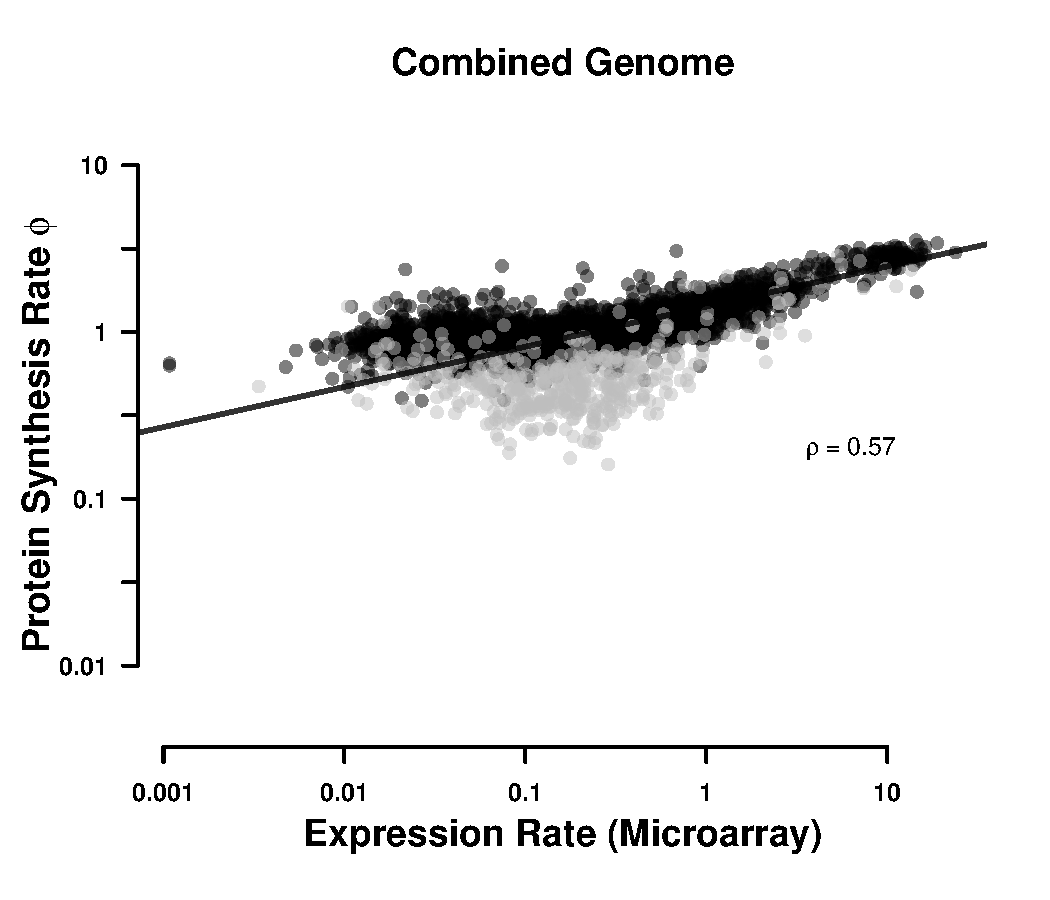
\includegraphics[width=.45\textwidth]{img/phi_corr_plot_whole_Genome_estim.pdf}
    \end{subfigure}
    \begin{subfigure}
        \centering
        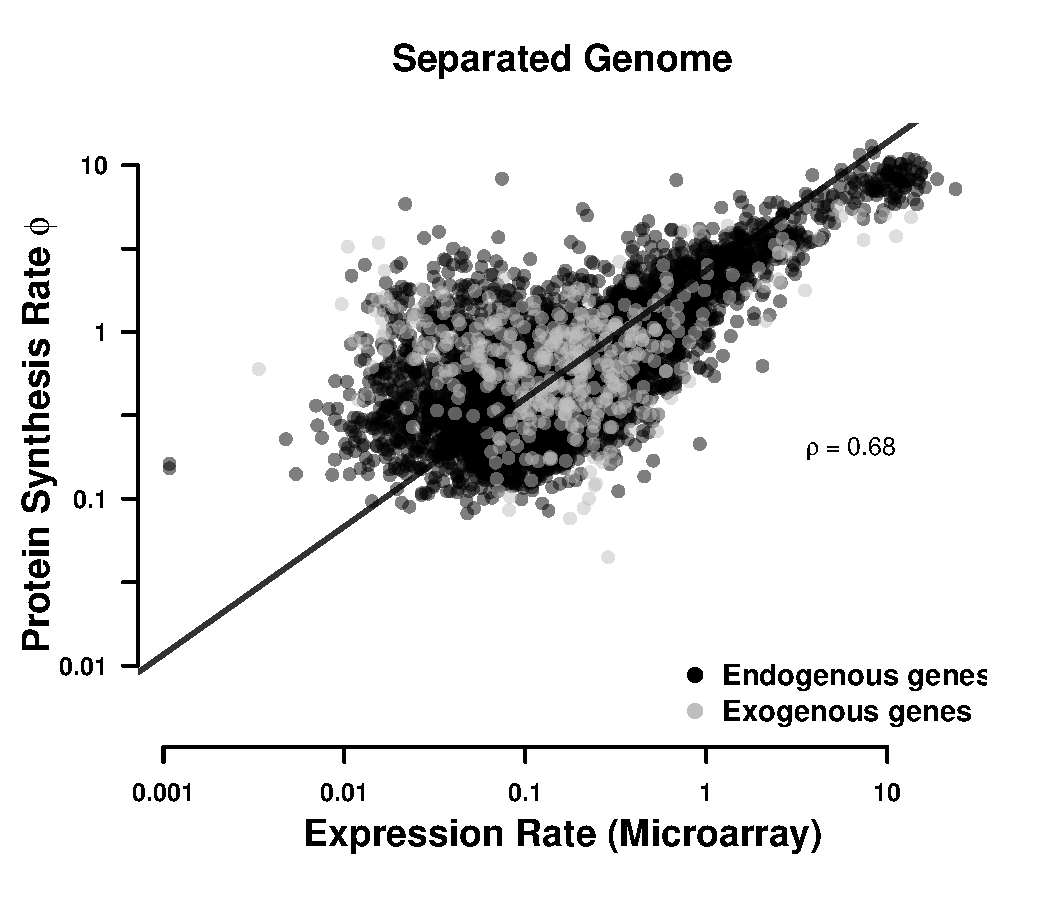
\includegraphics[width=.45\textwidth]{img/phi_corr_plot_split_Genome_estim.pdf}
    \end{subfigure}
    \caption{Comparison of predicted protein synthesis rate $\phi$ to Microarray data from XX for (a) the combined genome and (b) the separated endogenous and exogenous genes. Endogenous genes are displayed in black and exogenous genes in red. Black line indicates type II regression line.}
    \label{fig:phi_corr_two_cond}
\end{figure}

In addition to model selection, we utilized independent information on gene expression to evaluate model fit.
Recognizing differences in \DM and \DE for the endogenous and exogenous gene sets substantially improves our ability to predict protein synthesis rate $\phi$ ($\rho = 0.69$ vs. $\rho = 0.59$ for the full genome;  Figure \ref{fig:phi_corr_two_cond}).

\subsection*{Differences in the Endogenous and Exogenous Codon Usage}

As our estimates of parameters for a codon family coding for an amino acid are relative to a reference codon, changes in the reference codon will change the order between sets.
To better compare our estimates of of mutation bias (\DM) and selection bias (\DE) obtained from fitting \ROC between the endogenous and exogenous gene sets, we express our estimates relative to the mean for each codon family.
As 
We find larger differences between \DM than \DE (Figure \ref{fig:csp_comp}). 
Estimates of \DM in the endogenous genes negatively correlate with the \DM estimates for the exogenous genes ($\rho = -0.49$) indicating strong discordance in the mutation environment between \kluyveri and the donor lineage of the exogenous genes.
For example, $\sim 95 \%$ of codon families show mutation preference for A/T ending codons, in contrast, the exogenous genes display an equally strong mutation bias towards C/G ending codons.
Only the two codon amino acid Phenylalanine (Phe, F) shows complete concordance between endogenous and exogenous genes in their \DM values.
\begin{figure}[h]
    \centering
    \begin{subfigure}
        \centering
        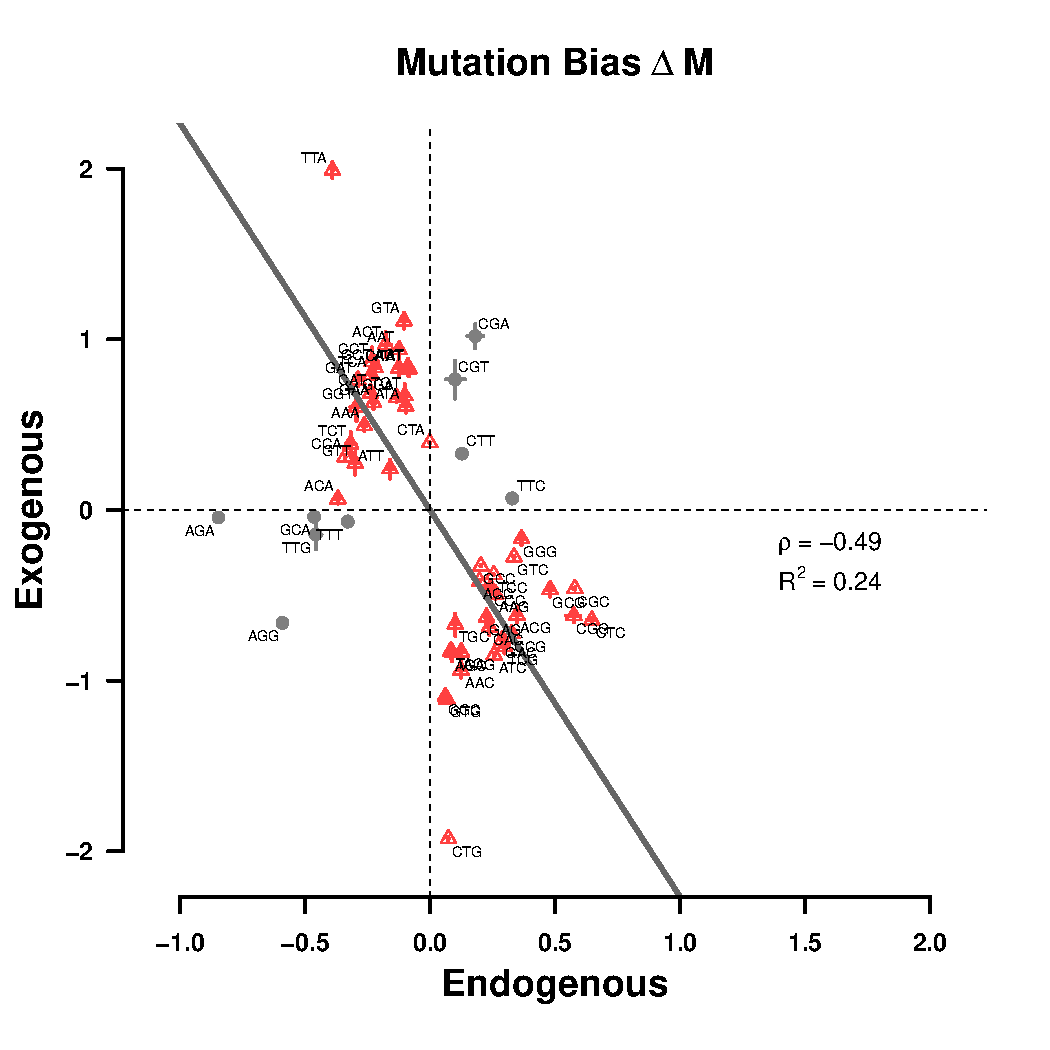
\includegraphics[width=.45\textwidth]{img/csp_corr_dm.pdf}
    \end{subfigure}
    \begin{subfigure}
        \centering
        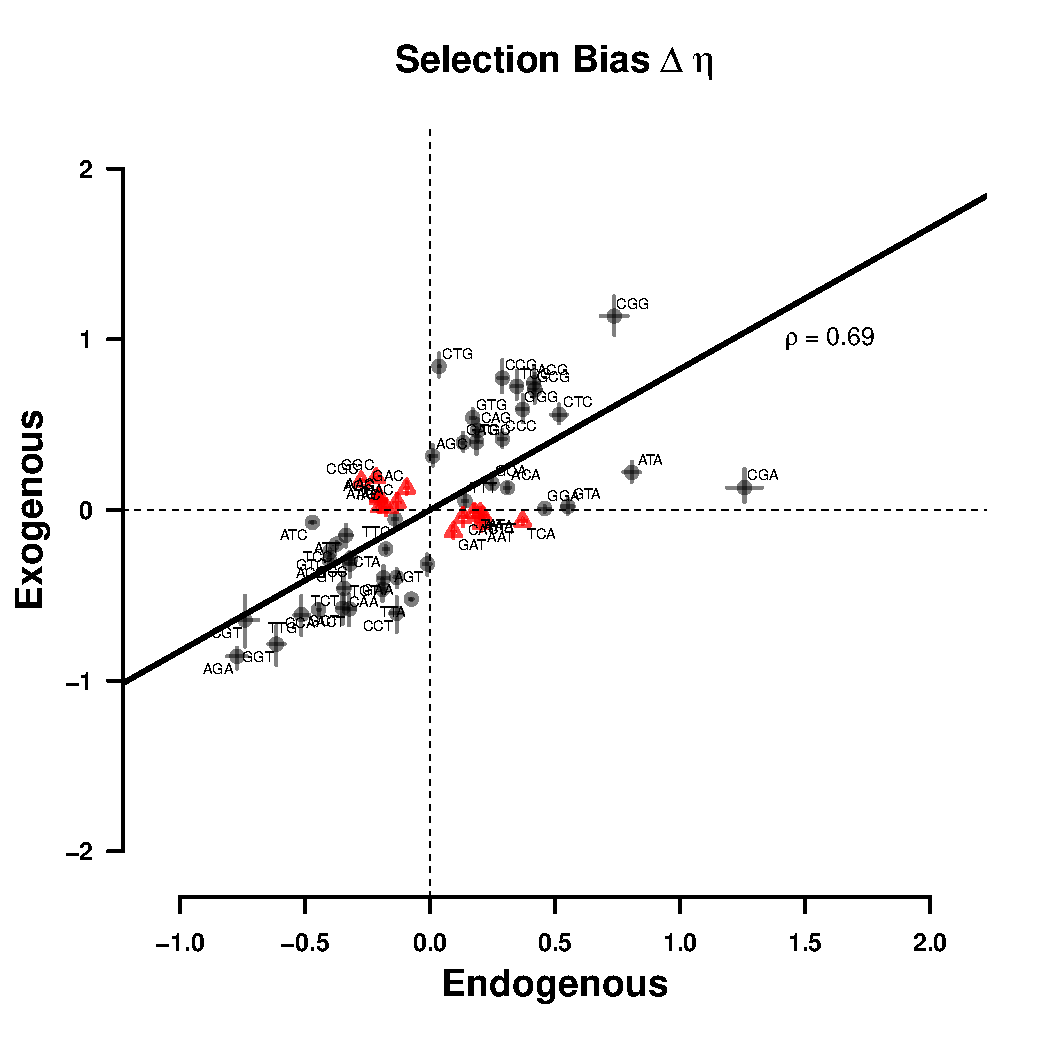
\includegraphics[width=.45\textwidth]{img/csp_corr_deta.pdf}
    \end{subfigure}
    \caption{Comparison of (a) mutation bias \DM and (b) selection bias \DE of endogenous and exogenous genes. Estimates are relative to the mean for each codon family. Black dots indicate parameters with sign concordance, red dots indicate parameters with sign discordance between endogenous and exogenous genes. Black line shows the type II regression. Dashed lines mark quadrants.}
    \label{fig:csp_comp}
\end{figure}

Estimates of \DE show higher agreement between endogenous and exogenous genes ($\rho = 0.69$) than our estimates of \DM.
However, only nine codon families favor the same codon in the endogenous and exogenous genes.
Unlike the mutation bias, we find selection to be heavily biased towards A/T ending codons ($\sim 89 \%$) in the exogenous genes.
In contrast, the selection environment in the endogenous genes is G/C biased ($\sim 58 \%$).

Under the null hypothesis, we assumed that $\DM_{exo} = \DM_{endo}$ and $\DE_{exo} = \DE_{endo}$.
We find that in that case, the codon most favored by mutation bias $\DM_{complete}$ is in concordance with the exogenous $\DM_{exo}$ estimates in 15 cases and in concordance with the endogenous $\DM_{endo}$ in only 3 cases (Table \ref{tab:codon_pref_dm}).
We find two cases, Isoleucine (Ile, I) and Arginine (Arg, R), in which the mutation preference of the complete genome is in discordance with both, the exogenous and the endogenous estimates.
Our estimate of the codon most favored by selection bias $\DE_{complete}$ are in concordance with the exogenous $\DE_{exo}$ estimates in 14 cases and are in concordance with the endogenous $\DE_{endo}$ in 13 cases (Table \ref{tab:codon_pref_deta}).
The estimated optimal codon between $\DE_{complete}$, $\DE_{exo}$, and $\DE_{endo}$ are in discordance for seven codon families.
Thus, recognizing and treating endogenous and exogenous genes as separate sets avoids the inference of incorrect synonymous codon preferences.

\subsection*{Determining Source of Exogenous Genes}

We combined our estimates of mutation bias ($\Delta M$) and selection bias ($\Delta \eta$) with synteny information and searched for potential source lineages of the introgressed region.
We examined 38 yeast lineages of which two (\emph{Eremothecium gossypii} and \emph{Candida dubliniensis}) showed a strong positive correlation in codon usage (Figure \ref{fig:csp_endo_exo_comp}a).
\begin{figure}[h]
    \centering
    \begin{subfigure}
        \centering
        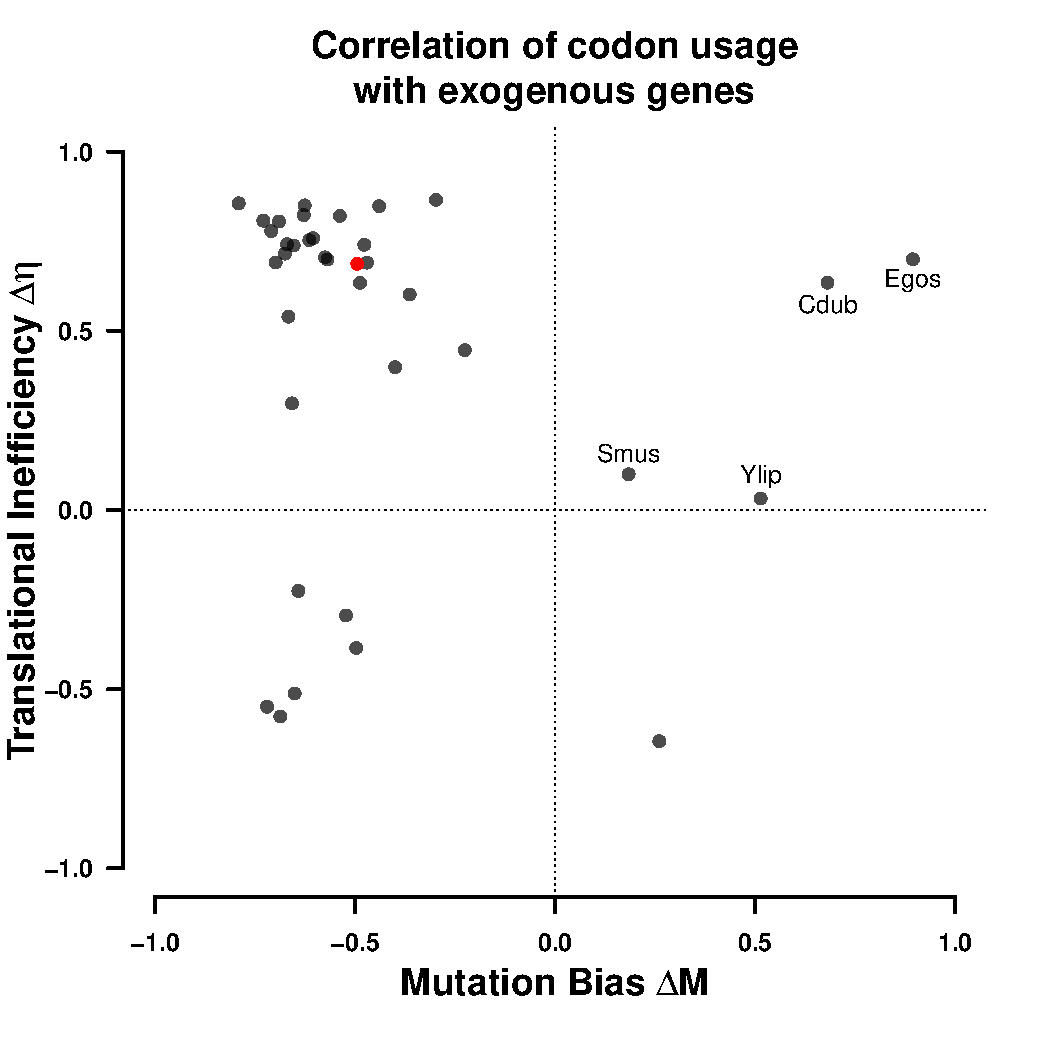
\includegraphics[width=.45\textwidth]{img/csp_mean_correlation_exo.pdf}
    \end{subfigure}
    \begin{subfigure}
        \centering
        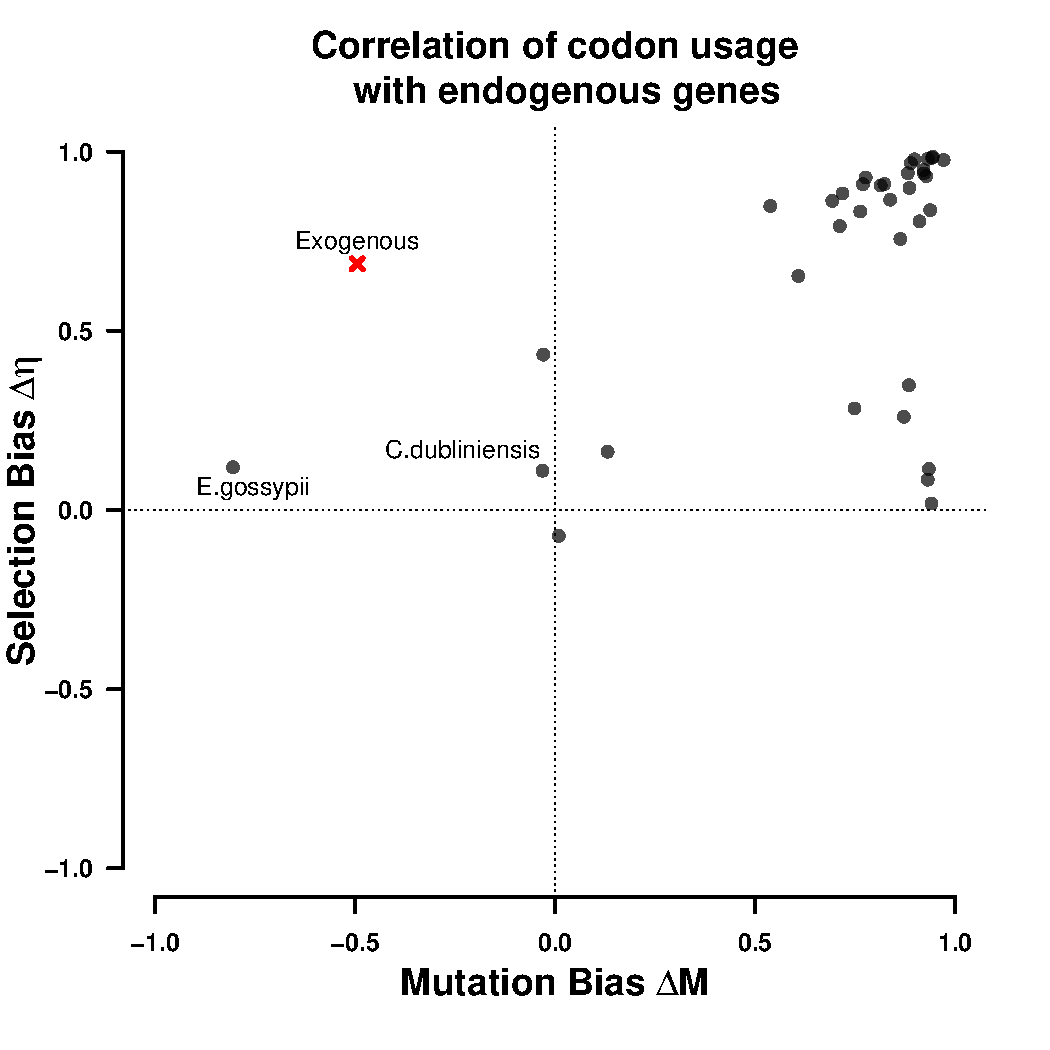
\includegraphics[width=.45\textwidth]{img/csp_mean_correlation_endo.pdf}
    \end{subfigure}
    \caption{Correlation of \DM and \DE of the (a) exogenous and (b) endogenous genes with 38 examined yeast lineages. Dots indicate the correlation of \DM and \DE of the lineages with the endogenous and exogenous parameter estimates. All regressions were performed using a type II regression.}
    \label{fig:csp_endo_exo_comp}
\end{figure}
The endogenous \kluyveri genome exhibits codon usage very similar to most yeast lineages examined, indicating little variation in codon usage among the examined yeasts (Figure \ref{fig:csp_endo_exo_comp}b).
Four lineages show a positive correlation for $\Delta M$ and $\Delta \eta$ with the exogenous genes and have a weak to moderate positive correlation in selection bias with the endogenous genes; but, like the exogenous genes, tend to have a negative correlation in $\Delta M$ with the endogenous genes.

Comparing synteny between the exogenous left arm of chromosome C, and \gossypii and \dubl as well as closely related yeast species we find that \gossypii displays the highest synteny coverage  (Figure \ref{fig:synteny_species}a,b).
\dubl, even though it displays similar codon usage does not show synteny with the exogenous region.
Furthermore, the synteny relationship between the exogenous region and other yeasts appears to be limited to the Saccharomycetacease group(Figure \ref{fig:synteny_species}b).
Given these results, we conclude that the \gossypii lineage is the most likely source of the introgressed exogenous genes.

\subsection*{Estimating Introgression Age}

We estimated the introgression age using an exponential model of decay for mutation bias, by assuming that \gossypii is still representative of the mutation bias of its ancestral source lineage at the time of the introgression.
We utilize the \DM estimates for all two codon amino acids and infer the age of the introgression to be on the order of $6.2\pm1.2\times 10^8$ generations. 
We assume a mutation rate of $3.8\times 10^{-10}$ per nucleotide per generation, a value in line with other estimates \citep{zhu2014, lang2008}.
\kluyveri experiences between one and eight generations per day, we therefore expect the introgression to have occurred about $205,000$ to $1,600,000$ years ago which is  longer than previous estimates of \citet{friedrich2015}.
However, our estimates are likely overestimates as they assume a purely neutral decay.

Furthermore, we estimated the persistence of the signal of the foreign cellular environment.
Assuming that differences in mutation bias will decay more slowly than differences in selection bias, we predict that the \DM signal of the source cellular environment will have decayed to be within one percent of the \kluyveri environment within about $5.4\pm0.2\times 10^9 $ generations.


\subsection*{Fitness Burden of the Exogenous Genes}

Estimates of selection bias for the exogenous genes show that, while well correlated with the endogenous genes, only nine amino acids share the optimal codon.
We therefore expect that the introgressed genes represent a significant reduction in fitness, or genetic load for \kluyveri, and even more so at the time of introgression.
As the introgression occurred before the diversification of \kluyveri and has fixed since then throughout the various populations, we are left without the original chromosome arm \citep{friedrich2015}.
However, using our estimates of $\Delta M$ and $\Delta \eta$ from the endogenous genes, we can estimate the genetic load of the exogenous genes relative to an expected gene set.
We define genetic load as the difference between the fitness of an expected, replaced endogenous gene and the inferred introgressed gene relative to drift $sN_e \propto \phi \DE$ (See Methods for details).
\begin{figure}[h]
    \centering
    \begin{subfigure}
        \centering
        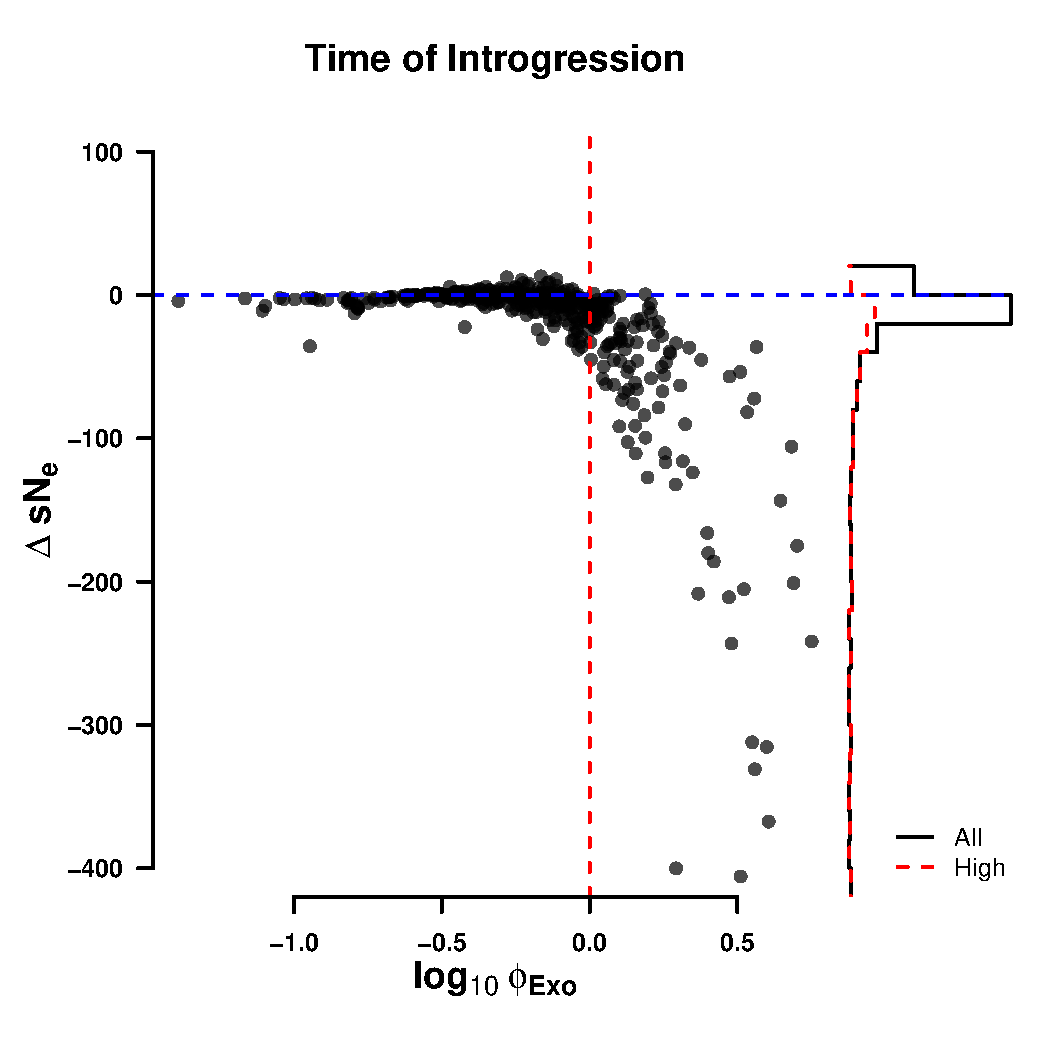
\includegraphics[width=.45\textwidth]{img/fitness_difference_gos_kappa5.pdf}
    \end{subfigure}
    \begin{subfigure}
        \centering
        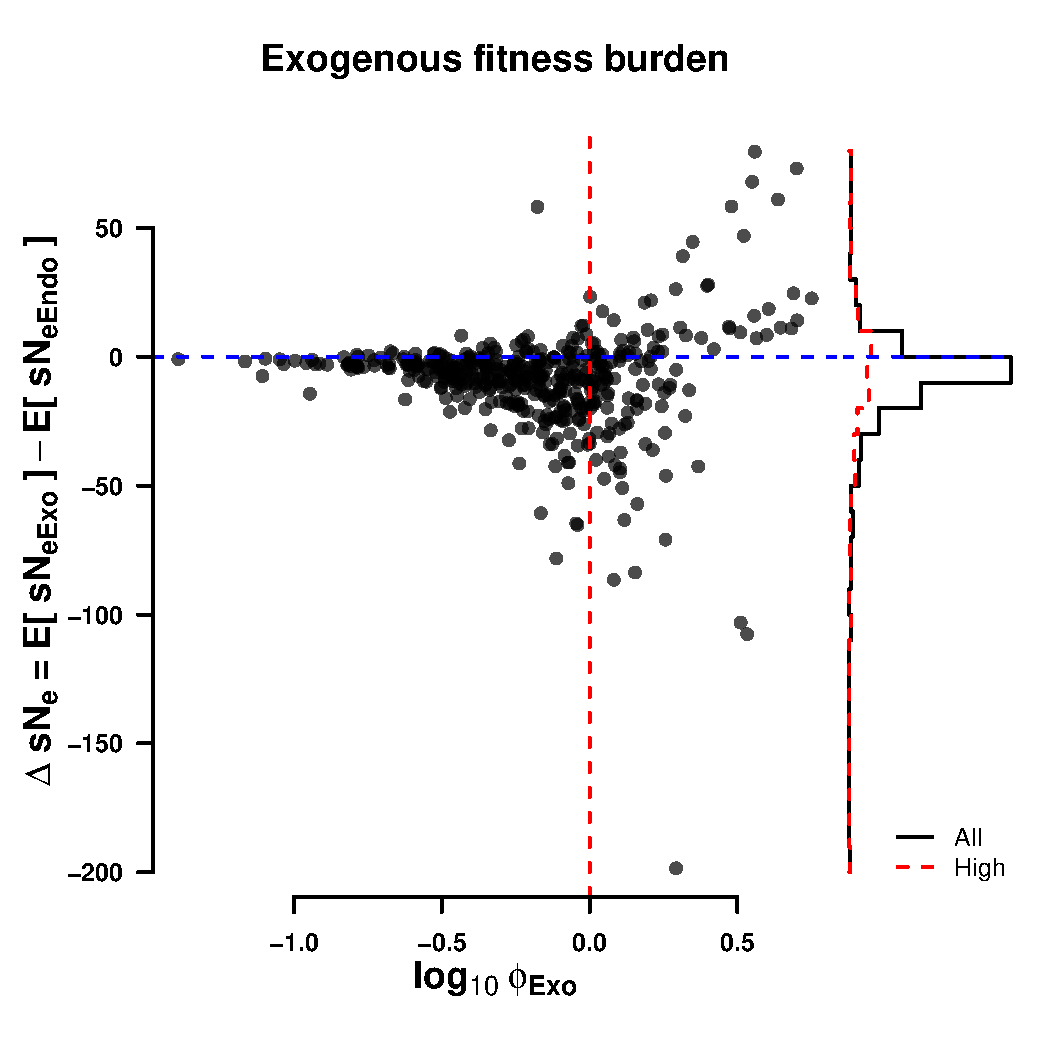
\includegraphics[width=.45\textwidth]{img/fitness_difference_exo.pdf}
    \end{subfigure}
    \caption{Fitness burden $\Delta sN_e$ (a) at the time of introgression ($\kappa = 5$), and (b) currently ($\kappa = 1$). }
    \label{fig:sne_fitness_burden}
\end{figure}

We estimate the genetic load of the exogenous genes at the time of introgression (Figure \ref{fig:sne_fitness_burden}a) and currently (Figure \ref{fig:sne_fitness_burden}b).
These estimates are dependent on three key assumptions.
First, we assume again that the current cellular environment of \gossypii is reflective of the ancestral environment.
Second, we assume that the current amino acid composition of the exogenous genes is the same as in the replaced endogenous genes.
Third, we assume that the difference in the efficacy of selection between \gossypii and \kluyveri can be described with a simple scaling term we call $\kappa$ (Figure \ref{fig:sne_scaling}b).
As \DE is defined as $\DE = 2N_eq(\eta_i-\eta_j)$, we can not distinguish if $\kappa$ is a scaling on protein synthesis rate $\phi$, effective population size $N_e$ the value of an ATP $q$\citep{gilchrist2015}.

At the time of the introgression, we predict that only a few genes were weakly exapted (Figure \ref{fig:sne_fitness_burden}a) with all high expression genes ($\phi > 1$) being maladapted to the novel cellular environment.
However, these highly expressed genes show the greatest rate of adaptation to the \kluyveri cellular environment (Figures \ref{fig:sne_fitness_burden}a, \ref{fig:adapt_tot}).

\section*{Discussion}

Using \ROC we show that the \kluyveri genome contains two distinct signatures of cellular environments, its own endogenous and a foreign exogenous one obtained by an introgression event ($\Delta AIC = 78,000$).
Following \citet{payen2009}, who defined the boundary of the anomalous chromosome region based on its elevated \GC, we partitioned the \kluyveri genome into an endogenous and an exogenous gene set using gene location.
We estimated the codon usage of the entire \kluyveri genome and the separated endogenous and exogenous gene sets (Figure \ref{fig:cub_all_sets}).
Both, Mutation bias and selection bias differ between endogenous and exogenous genes.
The endogenous genes show a strong mutation bias towards A/T ending codons, while the exogenous genes show mutation is bias towards G/C ending codons.
We observed the reversed to be true in selection bias, leading to a strong mismatch in codon usage between the gene sets, supporting our notion of two distinct signatures of codon usage.

Only half of the codon families share the same optimal codon in the endogenous and exogenous gene sets.
However, we find that the strength of selection within a codon family differs between gene sets, causing a change in rank order.
Nevertheless, we find a high correlation for our estimates of selection bias \DE between the two gene sets.
Our estimates of the optimal codon differ in nine cases between endogenous and exogenous genes.
Interestingly, when the difference in codon usage is ignored, we find that in seven out of these nine cases the exogenous codon preference is inferred as optimal(Table \ref{tab:codon_pref_deta}).
We find even greater discordance in our estimates of \DM between endogenous and exogenous gene sets(Table \ref{tab:codon_pref_dm}).
Without recognizing this difference in codon preference our estimates would not have been reflective of the actual codon usage of the \kluyveri genome but of a relatively small introgressed gene set.
This shows that a small number of exogenous genes ($\sim 9 \%$ of genes) can have a disproportional impact on our estimates of \DM and \DE when fitting \ROC to the entire \kluyveri genome.
While this is surprising, it highlights the importance to recognize differences in codon usage within a genome.
Our results also indicate that we can attribute the higher \GC in the exogenous genes mostly to differences in mutation bias favoring G/C ending codons rather than a novel selective force.

Separating the endogenous and exogenous genes improves our estimates of protein synthesis rate $\phi$ by $17 \%$ relative to the full genome estimate ($\rho = 0.59$ vs. $\rho = 0.69$, respectively).
Furthermore, we find that the variation in our estimates of $\phi$ is more consistent with the current understanding of gene expression (compare Figure \ref{fig:phi_corr_two_cond}a and b). 
Small variation in $\phi$ estimates may serve as an indicator for the presents of the signature of multiple cellular environments in future work.
In the case of the \kluyveri genome, finding a severe mismatch in \DM causes $\phi$ values for low expression genes ($\phi < 1$) to increase towards the inflection point where the dominance of mutation gives way to selection.
In the case of the two codon amino acids, the inflection point represents the point at which mutation and selection are contributing equally to the probability of a codons occurrence.
We find this inflection point around $\phi = 1$ for most amino acids (Figure \ref{fig:cub_all_sets}). 
However, \ROC assumes that estimates of $\phi$ follow a log-normal distribution with an expected value $E[\phi] = 1$. 
This assumption allows us to interpret \DE as the strength of selection relative to drift ($sN_e$) for a codon in a gene with the average protein synthesis rate $\phi = 1$.
However, tying the mean and standard deviation of the prior distribution together.
Therefore, an increase in $\phi$ for low expression genes has to be meet with a decrease of $\phi$ for high expression genes, reducing the overall variance in $\phi$ (see \citet{gilchrist2015} for details). 

Having shown that the introgressed exogenous genes reflect a foreign cellular environment, we used the quantitative estimates of mutation bias \DM and selection bias \DE from \ROC to identify potential source lineages.
The comparison of the endogenous and exogenous \DM and \DE estimates to 38 other yeast lineages revealed that most yeasts examined share similarity in mutation bias (Figure \ref{fig:csp_comp}).
Similar, we find strong similarities in selection bias between examined yeasts, potentially indicating stabilizing selection on codon usage.
However, the exogenous genes do not share this commonality (Figure \ref{fig:csp_comp}a), as their mutation bias strongly deviates from the endogenous genes and most other yeast species examined. 
This large difference in mutation bias between endogenous and exogenous genes allowed us to limit our candidate list to only two likely lineages, \dubl and \gossypii.
Interestingly, we did not find \emph{Lachancea thermotolerance}, a thermophilic lineage closely related to \kluyveri, as a potential candidate.
While \emph{L. thermotolerance} does have a strong synteny relationship with \kluyveri, it does not show similarity in codon usage with the exogenous genes and does not share their high \GC.

Inference of synteny relationships between the exogenous region and \dubl and \gossypii as well as closely related species showed that synteny relationship is limited to the Saccharomycetaceae clade (Figure \ref{fig:synteny_species}b).
\gossypii showed the highest syntenty coverage and is the only species with similar codon usage.
Furthermore, \gossypii is the only species examined with a \GC $> 50 \%$ like it is observed in the exogenous region.
The synteny coverage extends along the whole exogenous regions with the exception to the very 3' and 5' end of the region. 
The lack of synteny at the ends of the region also coincides with a drop in \GC, potentially indicating remains of the original replaced region or increased adaptation.
The ancestral introgressed region may have also broken up in \gossypii as we find non overlapping synteny with chromosomes \emph{VI} and \emph{V} as well as have indication that the C chromosome of \kluyveri very robust to recombination events \citep{payen2009, vakirlis2016}. 

With \gossypii identified as potential source lineage of the introgressed region, we inferred the time past since the introgression occurred using our estimates of mutation bias \DM.
The \DM estimates are well suited for this task as they are free of the influence of selection and unbiased by $N_e$ and other scaling terms, which is in contrast to our estimates of \DE \citep{gilchrist2015}.
We estimated the time since introgression to be on the order of $6\times 10^8$ generations, which is $\sim 10$ times longer time than a previous estimate by \citet{friedrich2015} of a minimum of $5.6\times 10^7$ generations .
However, our estimate implicitly assumes all mutations are neutral, it is therefore a conservative estimate, potentially overestimating the time since introgression. 
Our estimate also depend on the assumption that the \gossypii cellular environment reflects the ancestral environment at the time of the introgression.
If the the ancestral mutation environment was more similar to the \kluyveri environment at the time of the introgression than the \gossypii environment is today, we would overestimate this time.
On the other hand, we would underestimate the time since introgression if the two cellular environments were more dissimilar.
We could have attempted to reconstruct the ancestral state of \gossypii, however, as methods for ancestral state reconstruction are phenomenological, assumptions would be unclear. 

The estimates of mutation bias \DM also allow us the infer the time until the signature of the exogenous cellular environment will have decayed to be indistinguishable at about one percent difference.
Our estimate of decay is an order of magnitude greater than our estimate of the time since introgression ($5\times 10^9$ and $6\times 10^8$ generations).
Estimates of decay based on \DM are more conservative as we expect differences in \DE to decay before due to selection favoring the decay.
 
As we have determined that the introgression event has a long persisting exogenous signature, it is important to understand the fitness consequences of such an event.
We estimated the genetic load that the exogenous genes represent assuming that the replaced endogenous genes and the new exogenous genes had the same amino acid composition.
This assumption, along with the assumption that the current \kluyveri cellular environment is reflective of the cellular environment at the time of the introgression is necessary to estimate the expected endogenous sequence that was replaced.
Our results show that individual low expression genes contribute little to the genetic load, and show less adaptation to the novel cellular environment (Figure \ref{fig:sne_fitness_burden}, \ref{fig:adapt_tot}).
A small number of low expression genes even appear exapted, likely due to the mutation bias in the endogenous genes matching the selection bias in the exogenous genes for G/C ending codons.
Highly expressed genes on the other hand have greatly adapted to the \kluyveri cellular environment.
This, however, does not mean that these genes show a higher rate of evolution, but that small changes in their sequence have large impacts on the fitness burden these sequences represent.
To this day, the exogenous genes represent a significant fitness burden on \kluyveri.
However, our estimates are conservative as we do not account for potential changes in the codon usage of \gossypii. 
While divergent evolution in codon usage between \gossypii and \kluyveri would cause us to overestimate the genetic load, convergent evolution, on the other hand, would cause us to underestimate the genetic load.
However, as the introgression appears to have reached fixation \citep{friedrich2015}, the genetic load relative to the replaced chromosome arm is only of theoretical interest.

The large genetic load the exogenous genes represented at the time of the introgression indicates that the fixation of the introgression was a very unlikely event in a population with a large $N_e$ as it is typical for yeasts.
It is hard to contextualize the probability of this introgression being fixed as we are not aware of any estimates of the frequency at which such large scale introgressions of genes with very different signatures of codon usage occur.
One example is \emph{Saccharomyces bayanus}, a hybrid of \emph{Saccharomyces uvarum},\emph{Saccharomyces cerevisiae}, and \emph{Saccharomyces eubayanus}.
However, unlike with \kluyveri and \gossypii it appears that the donor lineages show similar codon usage.
\emph{Saccharomyces cerevisiae} and \emph{Saccharomyces eubayanus} show a very strong correlation between selection bias \DE of $\rho = 0.98$ and a strong correlation between mutation bias \DM of $ \rho = 0.83$
We were unable to identify codon usage for \emph{Saccharomyces uvarum}.
However, \kluyveri diverged about 85 Mya ago from the rest of the Lachancea clade.
This represents between $10^{10}$ to $10^{11}$ generations.
Assuming for yeasts typical effective population size on the order of $10^8$, we are left with $10^{18}$ to $10^{19}$ opportunities for such an event to occur.
In addition, the strong mutation bias towards G/C ending codons in the exogenous genes may have contributed to the fixation of this introgression (include figure of \DM v \DE).
It is, on the other hand, also possible that despite their mismatch in codon usage, the exogenous genes have represented a fitness increase due to external environmental factors resulting in the fixation of the introgression.
 
In conclusion, our results show the usefulness of the separation of mutation bias and selection bias and the importance of recognizing the presence of multiple cellular environments in the study of codon usage.
We also illustrate how a mechanistic model like \ROC and the quantitative estimates it provides can be used for more sophisticated hypothesis testing in the future.
In contrast to other approaches used to study codon usage like CAI \citep{sharp1987} or tAI \citep{dosreis2004}, \ROC is sensitive to differences in mutation bias.
We highlight potential pitfalls when estimating codon preferences, as estimates can be biased by the signature of a second, historical cellular environment.
In addition, we show how quantitative estimates of mutation bias and selection relative to drift can be obtained from codon data and used to infer the fitness cost of an introgression as well as its history and potential future.


\section*{Materials and Methods}

\subsection*{Separating endogenous and exogenous genes}
A GC-rich region was identified by \citet{payen2009} in the \kluyveri genome extending from position 1 to 989,693 of chromosome C.
This region was later identified as an introgression by \citet{friedrich2015}.
We obtained the \kluyveri genome from SGD Project \url{http://www.yeastgenome.org/download-data/} (last accessed: 09-27-2014) and the annotation for \kluyveri NRRL Y-12651 (assembly ASM14922v1) from NCBI (last accessed: 12-09-2014).
We assigned 457 genes located on chromosome C with a location within the $\sim 1 Mb$ window to the exogenous gene set.
All other 4864 genes of the \kluyveri genome were assigned to the exogenous genes.
All genes could be uniquely assigned to one or the other gene set.

\subsection*{Model Fitting with \ROC}
\ROC was fitted to each genome using AnaCoDa (0.1.1) \citep{landerer2018} and R (3.4.1).
\ROC was run from multiple starting values for at least 250,000 iterations, every 50th sample was collected to reduce autocorrelation. 
After manual inspection to verify that the MCMC had converged, parameter posterior means were estimated from the last 500 samples.

\subsection*{Comparing codon specific parameter estimates}
Choice of reference codon does reorganize codon families coding for an amino acid relative to each other, therefore all parameter estimates are relative to the mean for each codon family.
\begin{equation}
\DM_{i,a}^c = \DM_{i,a} - \bar{\DM_a}
\end{equation}
\begin{equation}
\DE_{i,a}^c = \DE_{i,a} - \bar{\DE_a}
\end{equation}
Comparison of codon specific parameters (\DM and \DE) was performed using the function lmodel2 in the R package lmodel2 (1.7.3) and R version 3.4.1.
Type II regression was performed with re-centered parameter estimates, accounting for noise in dependent and independent variable.


\subsection*{Synteny}
We obtained complete genome sequences from NCBI (last accessed: 02-05-2017).
Genomes were aligned and checked for synteny using SyMAP (4.2) with default settings \citep{soderlund2006, soderlund2011}.
We assessed Synteny as percentage non-overlapping coverage of the exogenous gene region (Figure \ref{fig:synteny_species}b).

\subsection*{Determining introgression timeline}
We modeled the change in codon frequency over time using an exponential model for all two codon amino acids, and describing the change in codon $c_1$ as
\begin{equation}
\frac{d c_1}{d t} = -\mu_{1,2}c_1 - \mu_{2,1}(1-c_1)
\label{mut_ode}
\end{equation}
where $\mu_{i,j}$ is the rate at which codon $i$ mutates to codon $j$ and $c_1$ is the frequency of the reference codon.
Our estimates of $\DM_{endo}$ can be directly related to the steady state of equation \ref{mut_ode}.
\begin{equation}
\frac{\mu_{2,1}}{\mu_{1,2} + \mu_{2,1}} = \frac{1}{1+\exp(\DM_{endo})}
\end{equation}
Solving for $\mu_{1,2}$ gives us $\mu_{1,2} = \DM_{endo}\exp(\mu_{2,1})$ which allows us to rewrite and solve equation \ref{mut_ode} as
\begin{equation}
c_1(t) = \frac{\exp(-t(1+\DM_{endo})\mu_{2,1})\exp(t(1+\DM_{endo})\mu_{2,1}) + (1+\DM_{endo})K}{1+\DM_{endo}}
\label{mut_close_form}
\end{equation}
where K is
\begin{equation}
K = \frac{-1 + c_1(0) + c_1(0)\DM_{endo}}{1+\DM_{endo}}
\end{equation}

Equation \ref{mut_close_form} was solved over time with a mutation rate $m_{2,1}$ of $3.8\times 10^{-10}$ per nucleotide per generation \citep{lang2008}. 
Initial codon frequencies $c_1(0)$ for each codon family where taken from our estimates of $\DM_{gos}$ from \gossypii. 
Current codon frequencies for each codon family where taken from our estimates of \DM from the exogenous genes.
Mathematica (9.0.1.0) \citep{Mathematica} was used to calculate the time $t_{exo}$ it takes for the initial codon frequencies $c_1(0)$ for each codon family to change to the current exogenous codon frequencies.
The same equation was used to determine the time $t_{endo}$ at which the signal of the exogenous cellular environment has decayed to within $1 \%$ of the endogenous environment.

\subsection*{Estimating fitness burden}

To estimate the fitness burden, we made three key assumptions.
First, we assumed that the current exogenous amino acid composition of genes is representative of the replaced endogenous genes.
Second, we assume that the currently observed cellular environment of \gossypii reflects the cellular environment that the exogenous genes experienced before transfer to \kluyveri.
Lastly, we assume that the difference in the efficacy of selection between the cellular environments of the source lineage and \kluyveri can be expressed as a scaling constant and that protein synthesis rate $\phi$ has not changed between the replaced endogenous and the introgressed exogenous genes.

We calculated the fitness burden each gene represents assuming additive fitness effects as 
\begin{equation}
(sN_e)_g = \sum_i^{C} -\kappa \phi_g \DE_i n_{g,i} 
\end{equation}
where $(sN_e)g$ is the selection against translation inefficiency relative to drift.
$\phi_g$ is the estimated protein synthesis rate for gene $g$ in the exogenous gene set.
$n_{g,i}$ is the codon count of each codon $i$ in the codon set $C$ for each gene $g$.
$\kappa$ is a constant, scaling the efficacy of selection between cellular environments.
Like stated previously, our \DE are relative to the mean of the codon family.
We find that the fitness burden of the introgressed genes  is minimized at $\kappa \sim 5$ (Figure \ref{fig:sne_scaling}b).
Thus, we set $\kappa = 1$ if we calculate the $(sN_e)g$ for the endogenous and the current exogenous genes, and $\kappa = 5$ for $(sN_e)g$ for the fitness burden at the time of introgression.
Since we are unable to observe codon counts for the replaced endogenous genes and for the exogenous genes at the time of introgression, we calculate expected codon counts
\begin{equation}
E[n_{g,i}] = \frac{\exp(-\DM_i -\DE_i\phi_g)}{\sum_j^C \exp(-\DM_j -\DE_j\phi_g)}\times m_{a_i}
\end{equation} 
$m_{a_i}$ is the number of occurrences of amino acid $a$ that codon $i$ codes for.

We report the fitness burden of the introgression as $\Delta sN_e = (sN_e)_{Intro} - (sN_e)_{Endo}$ where $(sN_e)_{Intro}$ is either the fitness burden at the time of the introgression or presently.

\section*{Acknowledgments}

This work was supported in part by NSF Awards MCB-1120370 (MAG and RZ) and DEB-1355033 (BCO, MAG, and RZ) with additional support from The University of Tennessee Knoxville. 
CL received support as a Graduate Student Fellow at the National Institute for Mathematical and Biological Synthesis, an Institute sponsored by the National Science Foundation through NSF Award DBI-1300426, with additional support from UTK. 
The authors would like to thank Brian C. O'Meara and Alexander Cope for their helpful criticisms and suggestions for this work.


\bibliographystyle{unsrtnat}
\bibliography{kluyveri_paper}

\clearpage
\section*{Supplementary Material}
\beginsupplement

Supporting Materials for \emph{Fitness consequences of mismatched codon usage} \ by Landerer \emph{et al.}.


\begin{table}
    \centering
\begin{tabular}{  l  c  c  c  c  }
\hline
	Amino Acid & \gossypii & Endogenous & Exogenous & \kluyveri \\ \hline \hline
	Ala A & GCG & GCA & GCG & GCG \\ \hline
	Cys C & TGC & TGT & TGC & TGC \\ \hline
	Asp D & GAC & GAT & GAC & GAC \\ \hline
	Glu E & GAG & GAA & GAG & GAG \\ \hline
	Phe F & TTC & TTT & TTT & TTT \\ \hline
	Gly G & GGC & GGT & GGC & GGC \\ \hline
	His H & CAC & CAT & CAC & CAC \\ \hline
	Ile I & ATC & ATT & ATC & ATA \\ \hline
	Lys K & AAG & AAA & AAG & AAA \\ \hline
	Leu L & CTG & TTG & CTG & CTG \\ \hline
	Asn N & AAC & AAT & AAC & AAT \\ \hline
	Pro P & CCG & CCA & CCG & CCG \\ \hline
	Gln Q & CAG & CAA & CAG & CAG \\ \hline
	Arg R & CGC & AGA & AGG & CGG \\ \hline
	Ser$_4$ S & TCG & TCT & TCG & TCG \\ \hline
	Thr T & ACG & ACA & ACG & ACG \\ \hline
	Val V & GTG & GTT & GTG & GTG \\ \hline
	Tyr Y & TAC & TAT & TAC & TAC \\ \hline
	Ser$_2$ Z & AGC & AGT & AGC & AGC \\ \hline
\end{tabular}
    \caption{Synonymous codon preference in the various data sets based on our estimates of $\Delta M$}
    \label{tab:codon_pref_dm}
\end{table}

\clearpage

\begin{table}
    \centering
\begin{tabular}{  l  c  c  c  c  }
\hline
	Amino Acid & \gossypii & Endogenous & Exogenous & \kluyveri \\ \hline \hline
	Ala A & GCT & GCT & GCT & GCT \\ \hline
	Cys C & TGT & TGT & TGT & TGT \\ \hline
	Asp D & GAT & GAC & GAT & GAT \\ \hline
	Glu E & GAA & GAA & GAA & GAA \\ \hline
	Phe F & TTT & TTC & TTC & TTC \\ \hline
	Gly G & GGA & GGT & GGT & GGT \\ \hline
	His H & CAT & CAC & CAT & CAT \\ \hline
	Ile I & ATA & ATC & ATT & ATT \\ \hline
	Lys K & AAA & AAG & AAA & AAG \\ \hline
	Leu L & TTA & TTG & TTG & TTG \\ \hline
	Asn N & AAT & AAC & AAT & AAC \\ \hline
	Pro P & CCA & CCA & CCT & CCA \\ \hline
	Gln Q & CAA & CAA & CAA & CAA \\ \hline
	Arg R & AGA & AGA & AGA & AGA \\ \hline
	Ser$_4$ S & TCA & TCC & TCT & TCT \\ \hline
	Thr T & ACT & ACC & ACT & ACT \\ \hline
	Val V & GTT & GTC & GTT & GTT \\ \hline
	Tyr Y & TAT & TAC & TAT & TAC \\ \hline
	Ser$_2$ Z & AGT & AGT & AGT & AGT \\ \hline
\end{tabular}
    \caption{Synonymous codon preference in the various data sets based on our estimates of $\Delta \eta$}
    \label{tab:codon_pref_deta}
\end{table}

\clearpage

\begin{figure}[h]
    \centering
    \begin{subfigure}
        \centering
        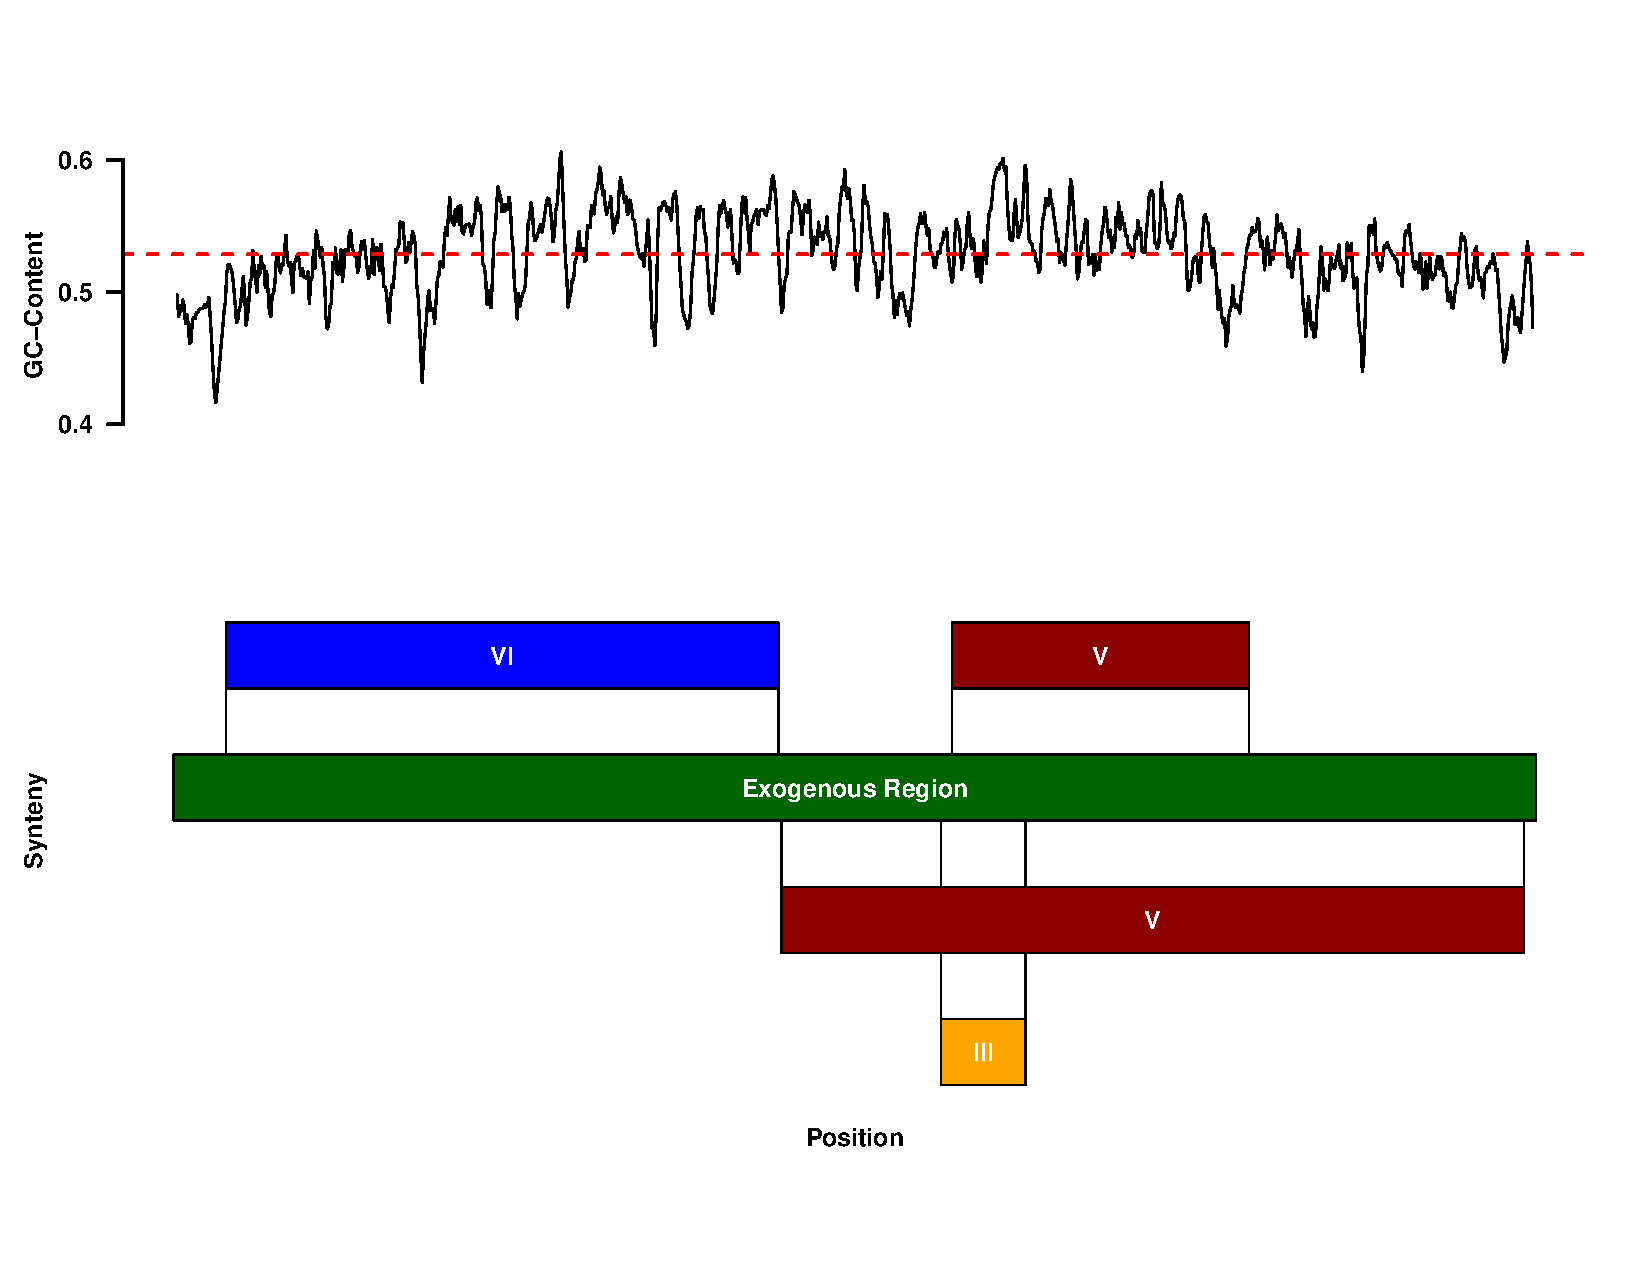
\includegraphics[width=.45\textwidth]{img/synteny_blocks_and_gc.pdf}
    \end{subfigure}
    \begin{subfigure}
        \centering
        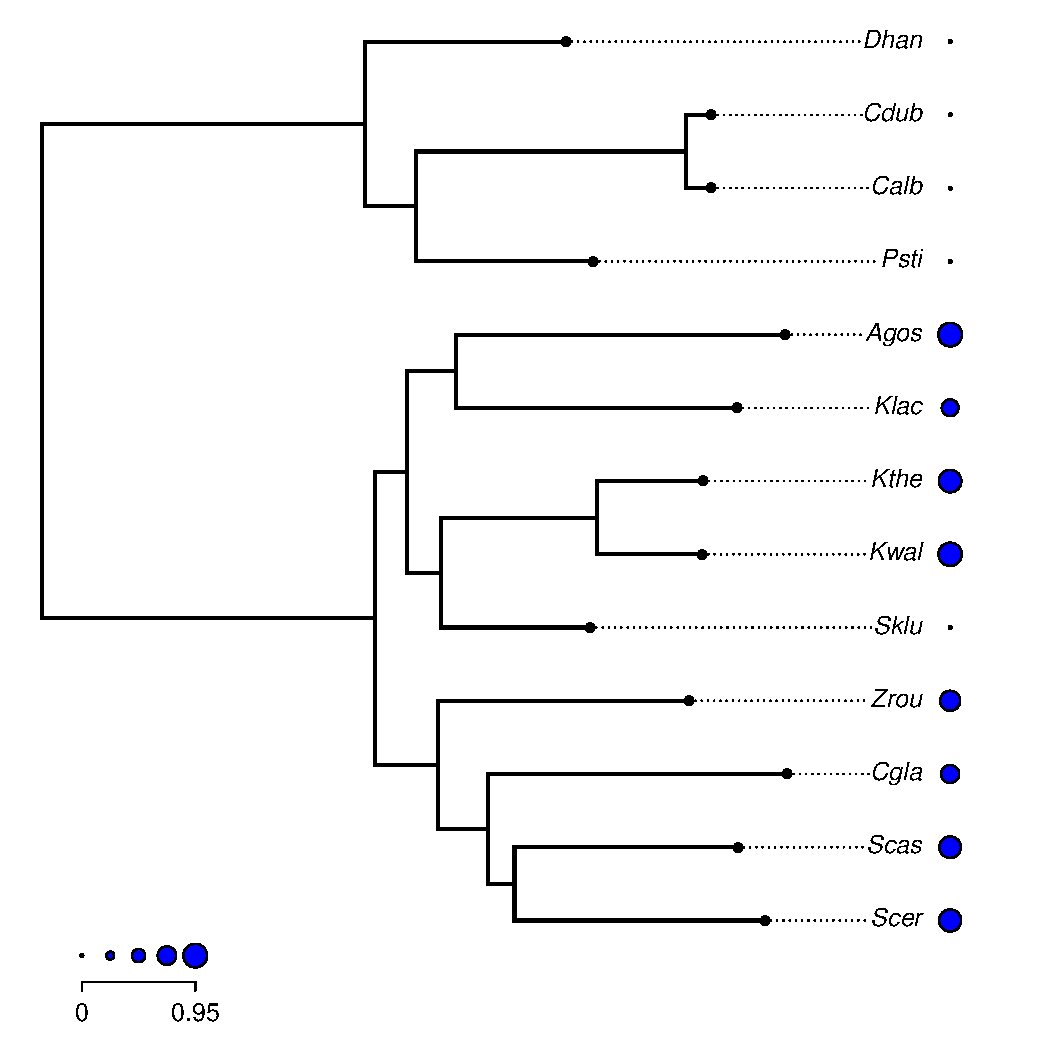
\includegraphics[width=.45\textwidth]{img/synteny_coverage.pdf}
    \end{subfigure}
    \caption{Suppl Fig: Synteny relationship of \gossypii and the exogenous genes (left), Amount of synteny for each species (Units of std dev) checked for synteny.}
    \label{fig:synteny_species}
\end{figure}

\begin{figure}[h]
    \centering
    \begin{subfigure}
        \centering
        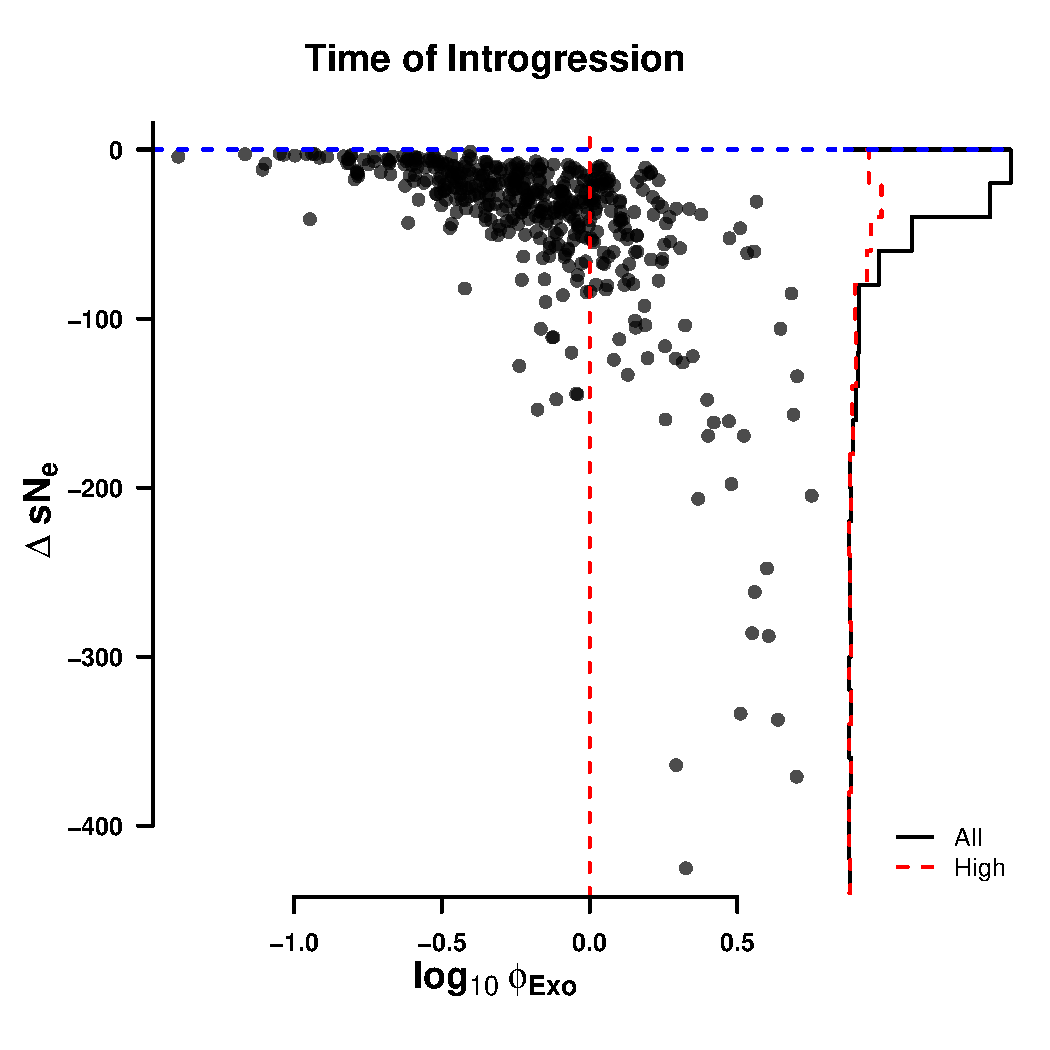
\includegraphics[width=.45\textwidth]{img/fitness_difference_gos_kappa1.pdf}
    \end{subfigure}
    \begin{subfigure}
        \centering
        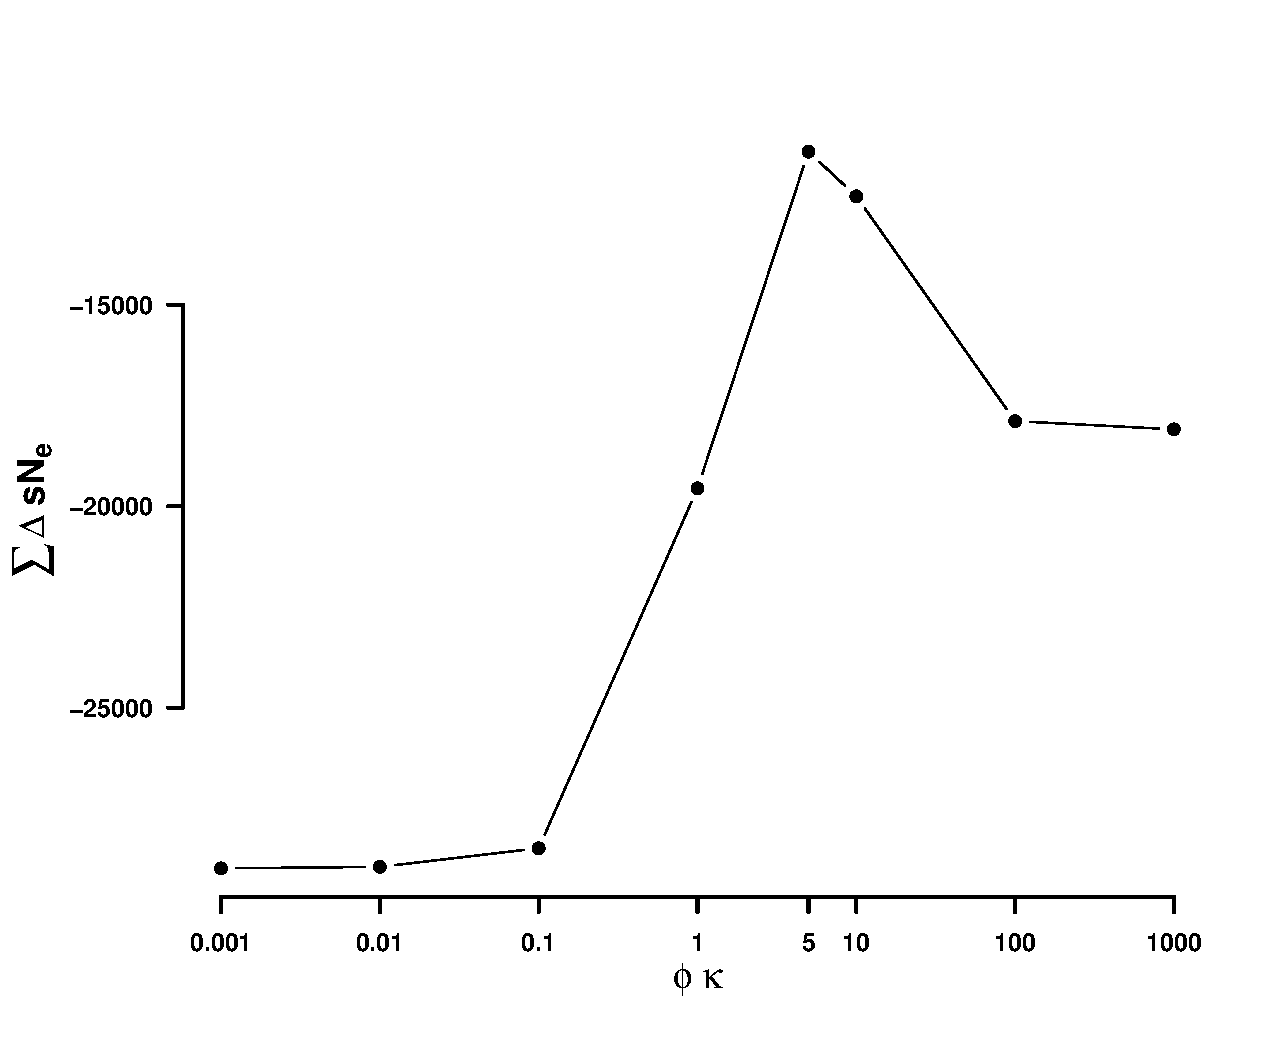
\includegraphics[width=.45\textwidth]{img/fitness_phi_scaling_gos.pdf}
    \end{subfigure}
    \caption{Suppl Fig: Fitness burden (left) without scaling of $\phi$, and change of total fitness burden with scaling $\kappa$}
    \label{fig:sne_scaling}
\end{figure}

\begin{figure}[H]
     \centering
	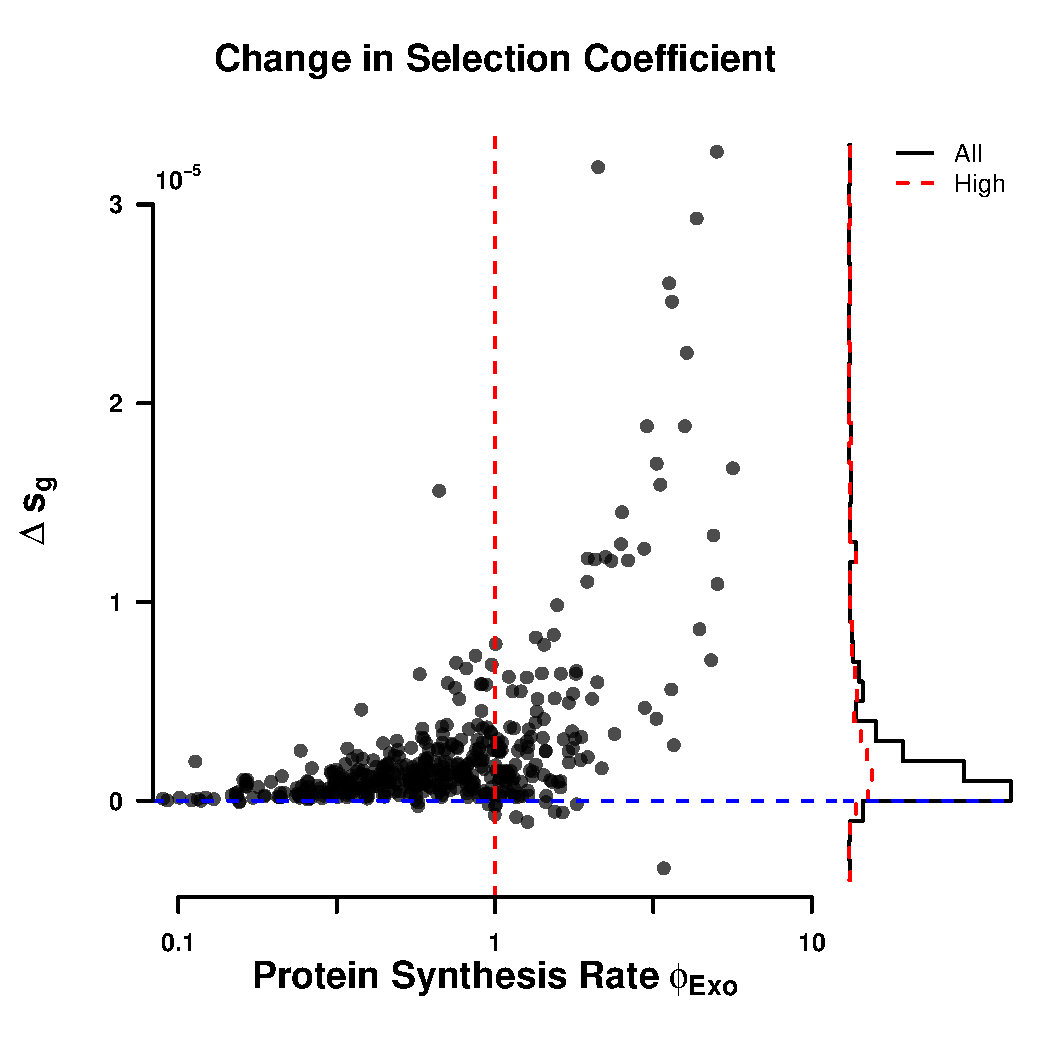
\includegraphics[width=\textwidth]{img/adaptation_total.pdf}
	\caption{Total amount of adaptation between time of introgression and now}
	\label{fig:adapt_tot}
\end{figure}

\clearpage
\begin{figure}[H]
     \centering
	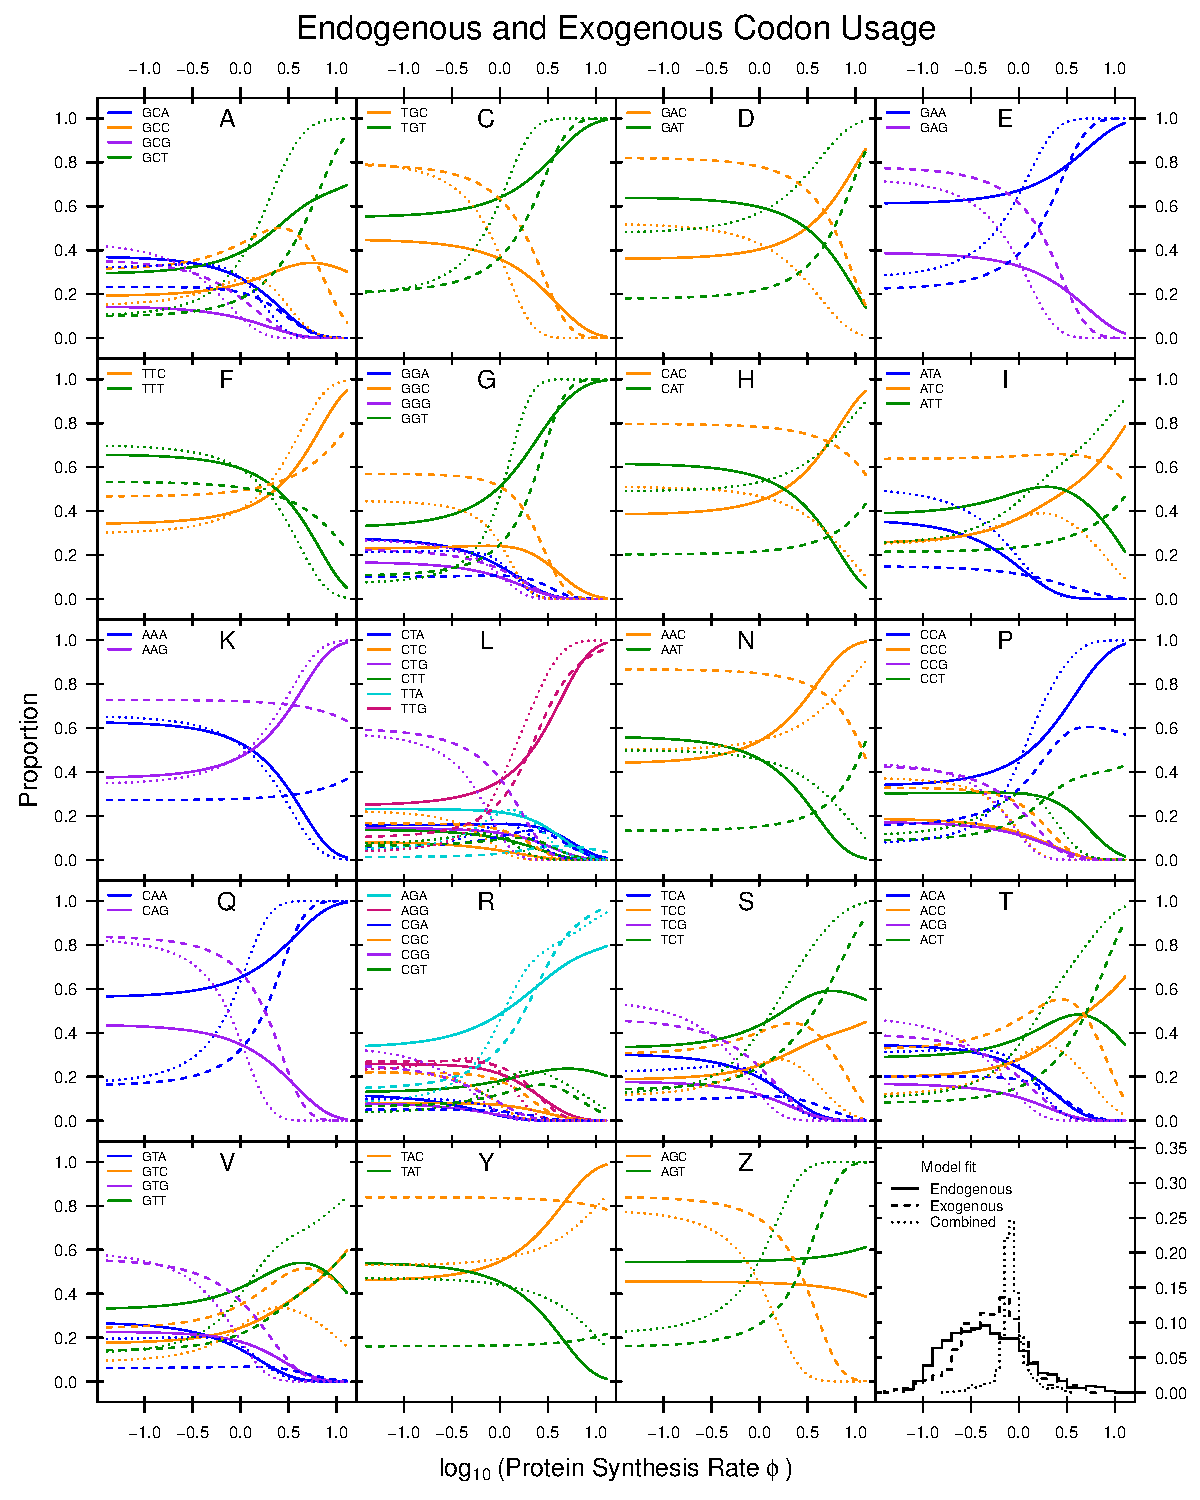
\includegraphics[width=\textwidth]{img/CUB_cleft_main.pdf}
	\caption{Suppl Fig}
	\label{fig:cub_all_sets}
\end{figure}

\end{document}
